\documentclass{beamer}
%
% Choose how your presentation looks.
%
% For more themes, color themes and font themes, see:
% http://deic.uab.es/~iblanes/beamer_gallery/index_by_theme.html
%

% Theme License: https://creativecommons.org/licenses/by/4.0/

\mode<presentation>
{
  \usetheme{metropolis}   % https://github.com/matze/mtheme
  \usecolortheme{default} % or try albatross, beaver, crane, ...
  \usefonttheme{default}  % or try serif, structurebold, ...
  \setbeamertemplate{navigation symbols}{}
  \setbeamertemplate{caption}[numbered]
} 

\usepackage[english]{babel}
\usepackage[utf8x]{inputenc}

\title[Ghidra]{An Introduction to Reverse Engineering}
\author{Jake Vossen}
\institute{Colorado School of Mines - oresec}
\date{2019-03-19}

\begin{document}

\begin{frame}
  \titlepage
\end{frame}

% Uncomment these lines for an automatically generated outline.
%\begin{frame}{Outline}
%  \tableofcontents
%\end{frame}

\section{Introduction}

\begin{frame}{What is Software Reverse Engineering?}

\begin{itemize}
  \item IEEE defines it as ``he process of analyzing a subject system to identify the system's components and their interrelationships and to create representations of the system in another form or at a higher level of abstraction''
  \item Generally is taking a piece of compiled software and analyzing
    it, revealing information about the source code
  \item Often used in security research, but also have implication in
    game emulation and other areas of proprietary software
  \item Also used to analyze malware to create figure out how to get
    around ransomware and other attacks
\end{itemize}

\vskip 1cm

\end{frame}

\begin{frame}{Why Ghidra?}
  \begin{figure}
    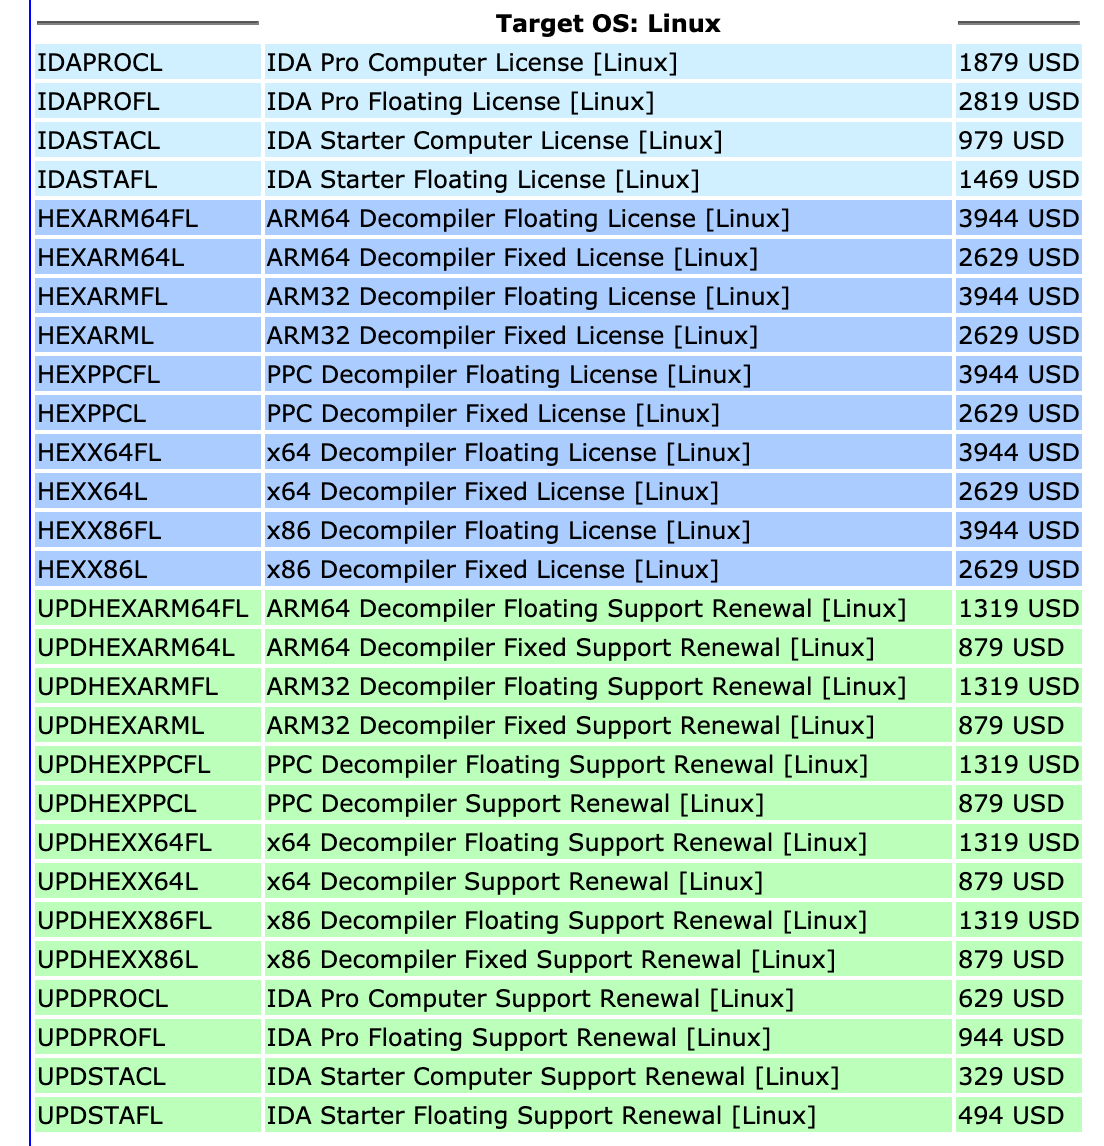
\includegraphics[width=\textwidth]{hex-rays-pricing.png}
    %% \caption{\label{fig:your-figure}Hex Rays Pricing}
  \end{figure}
\end{frame}

\begin{frame}{And if that wasn't enough...}
  \begin{figure}
    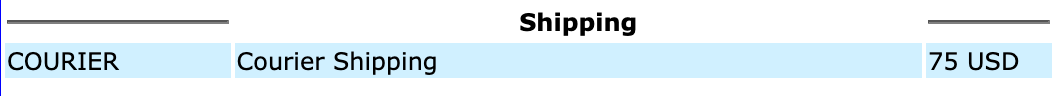
\includegraphics[width=\textwidth]{ida-shipping.png}
    %% \caption{\label{fig:your-figure}Hex Rays Pricing}
  \end{figure}
\end{frame}

\begin{frame}{And Ghidra...}
  \begin{itemize}
    \item Free and open source - Apache 2.0 Licensed or Public Domain
      (choice of contributor)
      \url{https://github.com/NationalSecurityAgency/ghidra}
    \item Has a lot better support for people working on teams then
      IDA 
    \item Security professionals are saying it rivals the
      functionality of IDA
  \end{itemize}
\end{frame}

% Commands to include a figure:
%\begin{figure}
%\includegraphics[width=\textwidth]{your-figure's-file-name}
%\caption{\label{fig:your-figure}Caption goes here.}
%\end{figure}

\section{Compiler Theory (a 10,000 foot overview)}

\begin{frame}{What are the Goals of a compiler?}
  \begin{itemize}
    \item Take a programming language that is human-readable and
      writable, into something that the computer can run.
    \item Generally a program is considered compiled if it is in
      assembly code - assembly to machine code is done by a
      \textit{assembler}, not a compiler.
    \item Three parts: parsing, type checking, and code
      generation. [1]
    \item Optionally, you can improve the efficiency as you do this
  \end{itemize}
\end{frame}

\begin{frame}{Wait, how do decompilers work anyways? Or even a
    compiler?}
  \begin{itemize}
    \item Option A: Compile down into another
      language to be run. GNU yacc and bison are intermediate
      languages and parsers where you can define your new programming
      language and generate machine code from it.
    \item Option B (generally better): Compiler is written in the
      language itself.
  \end{itemize}
\end{frame}

\begin{frame}{How are compilers born for language X?}
  Problem: We want a compiler that can compile the compiler.

  Solutions:
  \begin{itemize}
    \item Write a compiler for X in language Y. Now that we have an X
      compiler, rewrite the compiler in X itself
    \item Expand on an existing programming language and use it's compiler
    \item Write the compiler in X, hand compile it, now you have a
      compiler
  \end{itemize}
  So the very first compilers where written \textbf{by hand} in
  assembly. 
\end{frame}

\section{Decompiler Theory (100,000 foot overview)}

\begin{frame}{Why are decompilers are harder and more limited?}

  People do their best, but decompiling is even harder than
  compiling, which is already a really hard problem. Some of the
  things that make it harder is:
  
  \begin{itemize}
    \item Types are in the hidden, instead of being in plain text in
      the language.
    \item If something isn't formatted the way you want, you can't
      just throw and error like compiling.
    \item Output has to be human readable and clean, compared to
      assembly which
    \item Exception handling
  \end{itemize}

  Things like tail end recursion and stack/heap variable ranges are
  just too difficult sometimes, so decompiling is not
  perfect. Generally, it will result in ``equivalent'' code, not
  necessarily the the original code.
\end{frame}

\begin{frame}{What are the steps decompilers take?}

%  It is similar to the steps that a compiler takes in reverse, but
%  that generates worse code, so some other steps are thrown in

  \begin{itemize}
    \item Generate microcode: a step between machine code and
      assembly. This lets us do some optimization before we translate
      further
    \item Optimization: The microcode is verbose, so we need to clean
      it up a bit. This is done at a local (inside a
      function/subroutine) to a global level. This results in a more
      readable end result.
    \item Structural analysis: Look at our microcode and figure out
      where we are looping, jumping, etc to create a control flow
      graph
    \item Pseudocode generation: Generate the output from the
      optimization and structural analysis. After this is complete, we
      also have to optimize and clean it up, as it still may be too
      verbose.
    \item Type analysis: Black magic analysis of the pseudocode
  \end{itemize}
\end{frame}

\section{Installing and setting up Ghidra}
\begin{frame}{Tin Foil Hats...}

  Yes, you are going to be installing software from the NSA. People
  have already been searching for backdoors and other shenanigans, and
  nobody has found anything. The source code should be released in the
  next couple days. The NSA has over 30 open source projects[2],
  including things that have been merged into Android and some Linux
  distributions like Red Hat.
\end{frame}

\end{document}

% [1] http://steve-yegge.blogspot.com/2007/06/rich-programmer-food.html
% [2] https://code.nsa.gov/